% Auto-generated by make_pretraining_diagnostics.py — do not edit by hand.
% Section: Why recon-only training cannot price.

\subsection{Why recon-only training cannot price}
\label{subsec:why_pretraining_cannot_price}

This subsection assembles the empirical evidence that the encoder--decoder
checkpoints from Chapter~\ref{chap:encoderdecodermodel} cannot, on their own,
price ATM swaptions by Monte Carlo. The discussion separates two distinct
failures that occupy the same symbol: the \emph{simulation} failure of
the unconstrained drift in the baseline architecture, and the \emph{decoding}
failure of the recon-only decoder when fed simulated latent states.

\paragraph{The pricing pipeline as a probe.}
The pricing pipeline of Section~\ref{sec:swaption_pricing_methodology} can
be read as a stress test. From an encoded $z_0$, Euler--Maruyama is run
forward to expiry to obtain $z_T$, and the decoder maps $z_T$ to a
discount curve. Recon-only training optimises the decoder only on the
manifold $\{\mathrm{encoder}(x) : x \in \mathcal{X}_{\mathrm{train}}\}$,
which is a measure-zero subset of $\mathbb{R}^\ell$. Anything outside
this manifold is uncharted territory, and Brownian increments push $z_T$
off the manifold immediately.

\paragraph{Decoder robustness to off-manifold inputs.}
We probe each decoder directly by perturbing encoded points
$z = z_0 + \varepsilon \eta$, $\eta \sim \mathcal{N}(0, I_\ell)$, and
measuring the fraction of decoded curves $\mathcal{G}(z)$ that are
fully finite. Figure~\ref{fig:decoder_robustness} and
Table~\ref{tab:decoder_robustness} show that recon-only decoders break down
sharply for $\varepsilon \gtrsim 0.5$. The stable variant is in fact
\emph{more} robust than baseline at every scale tested
(dim4 stable decodes 48.4\% at $\varepsilon = 0.5$ versus
18.0\% for baseline), but no recon-only decoder is reliable far
from its training manifold.

\begin{figure}[H]
    \centering
    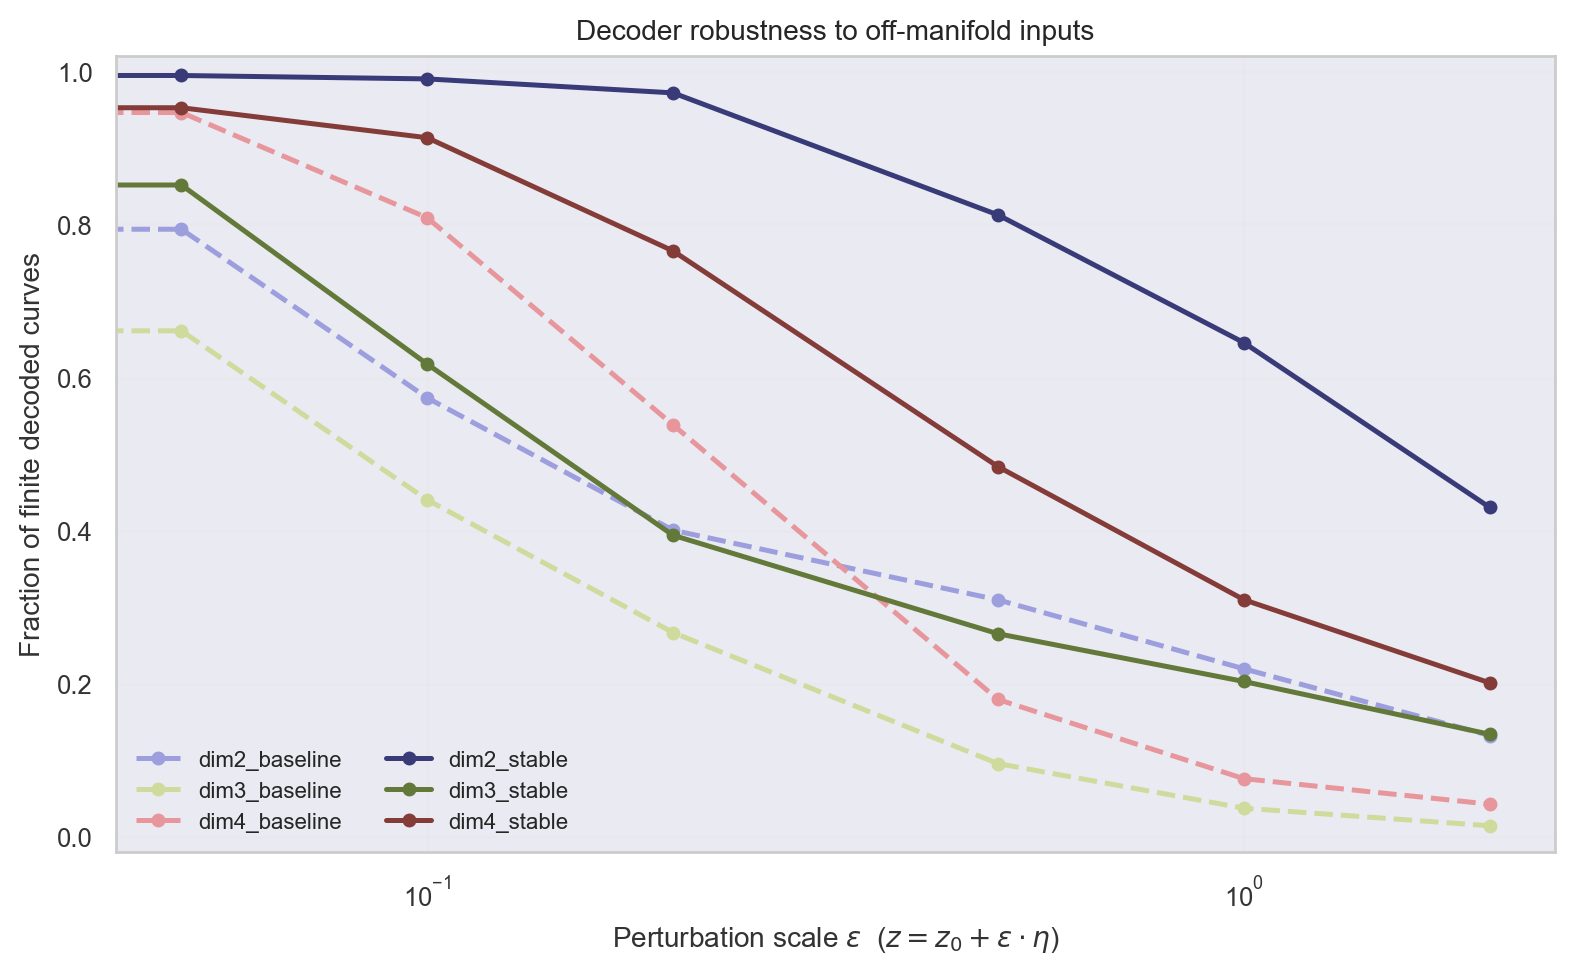
\includegraphics[width=0.85\textwidth]{Figures/Pricing/fig_decoder_robustness.png}
    \caption{Decoder finite-decoding fraction versus isotropic perturbation
    scale $\varepsilon$. Stable decoders are uniformly more robust than
    baseline decoders of the same dimension, but all decoders fail rapidly
    beyond $\varepsilon \approx 0.5$.}
    \label{fig:decoder_robustness}
\end{figure}

\begin{table}[H]
\centering
\caption{Fraction of decoded discount curves that are fully finite, as a function of perturbation scale $\varepsilon$. Each cell averages over 200 EUR curves $\times$ 50 isotropic Gaussian draws $= 10{,}000$ test points. All decoders handle $\varepsilon = 0$ perfectly (on-manifold); robustness degrades sharply for displacements above $\varepsilon \approx 0.5$.}
\label{tab:decoder_robustness}
\small
\begin{tabular}{lrrrrrrr}
\toprule
Model & $\varepsilon = 0.0$ & $\varepsilon = 0.05$ & $\varepsilon = 0.1$ & $\varepsilon = 0.2$ & $\varepsilon = 0.5$ & $\varepsilon = 1.0$ & $\varepsilon = 2.0$ \\
\midrule
\texttt{dim2_baseline} & 1.000 & 0.794 & 0.574 & 0.401 & 0.310 & 0.220 & 0.132 \\
\texttt{dim3_baseline} & 1.000 & 0.661 & 0.440 & 0.267 & 0.096 & 0.038 & 0.015 \\
\texttt{dim4_baseline} & 1.000 & 0.946 & 0.809 & 0.538 & 0.180 & 0.076 & 0.043 \\
\texttt{dim2_stable} & 1.000 & 0.995 & 0.990 & 0.972 & 0.812 & 0.646 & 0.430 \\
\texttt{dim3_stable} & 1.000 & 0.852 & 0.618 & 0.394 & 0.265 & 0.203 & 0.134 \\
\texttt{dim4_stable} & 1.000 & 0.952 & 0.913 & 0.765 & 0.484 & 0.310 & 0.201 \\
\bottomrule
\end{tabular}
\end{table}

\paragraph{Where the SDE actually goes.}
Whether the recon-only decoder's finite-frac is reached during real
simulation depends on the SDE's displacement distribution. Simulating
1{,}000 EM paths to $T_e = 5$Y from a representative EUR curve
(Figure~\ref{fig:latent_displacement_cdf},
Figure~\ref{fig:latent_displacement_scatter}, and
Table~\ref{tab:displacement_summary}) reveals two qualitatively different
pathologies in the dim4 case. The baseline SDE diverges to
$\|z_T - z_0\| \sim 3.9e+13$ — thirteen orders of magnitude
larger than the stable SDE's $\|z_T - z_0\| \sim 2.2$.
At those astronomical magnitudes, the baseline decoder happens to extrapolate
to finite-but-meaningless outputs, returning curves that yield the
$+200$ to $+2000$ basis-point pricing errors documented in
Table~\ref{tab:baseline_pricing_errors}.\footnote{The label
\texttt{tab:baseline\_pricing\_errors} refers to the per-cell pricing-error
table; substitute the correct label if it differs in this thesis.}
The stable decoder rejects its (well-behaved) inputs with a NaN
(51\% finite), because $\|z_T - z_0\| \approx 2$ is squarely in
the regime where Figure~\ref{fig:decoder_robustness} predicts decoder
failure. Two different broken things, one common consequence: recon-only
training cannot price.

\begin{figure}[H]
    \centering
    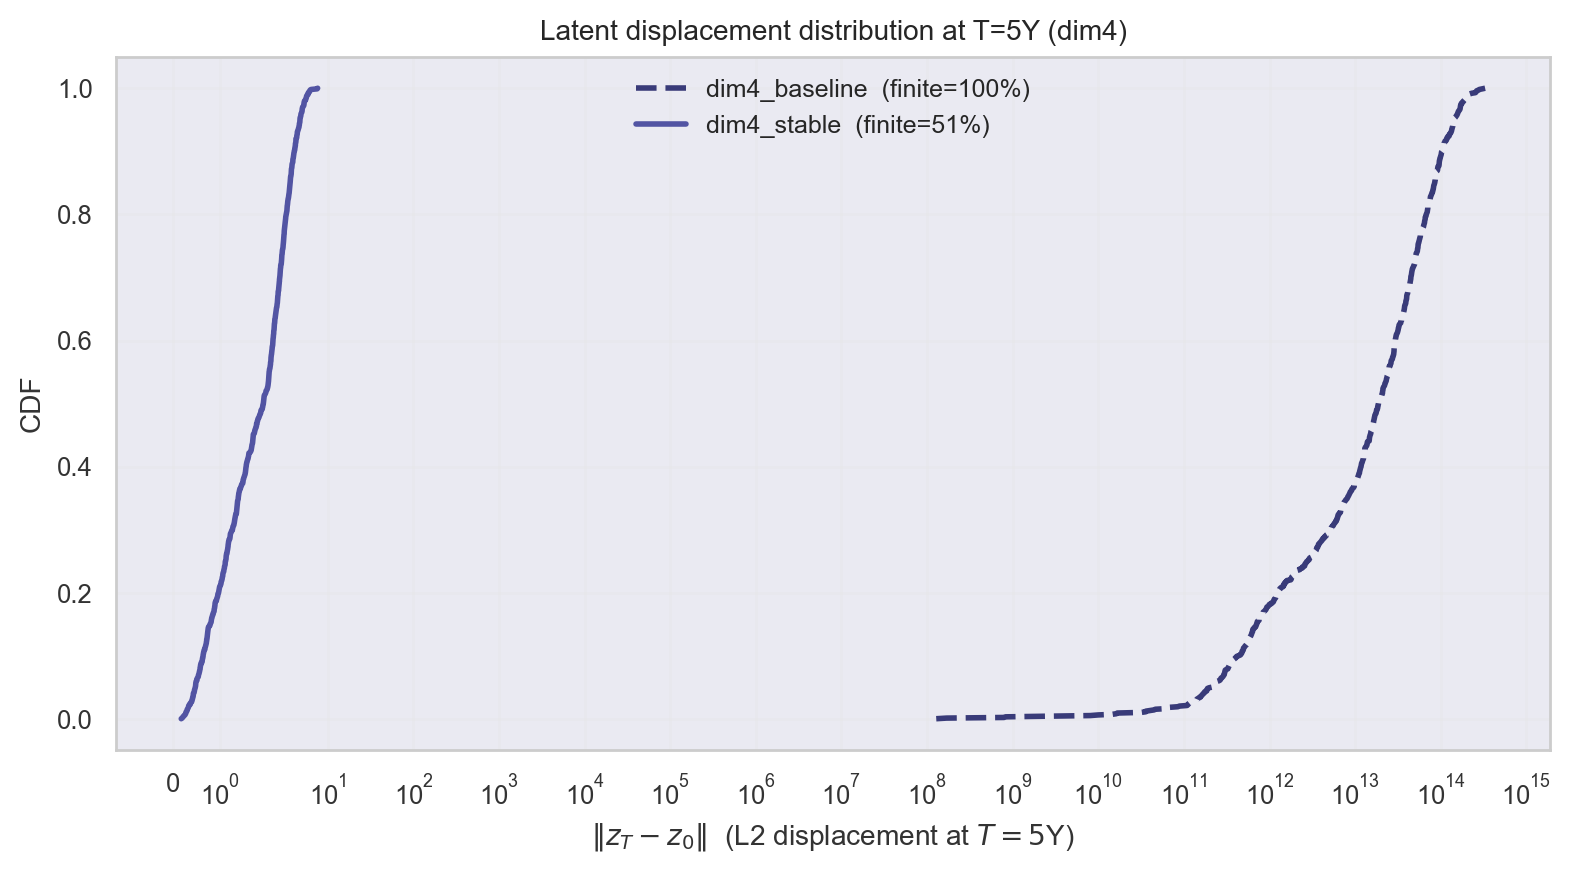
\includegraphics[width=0.85\textwidth]{Figures/Pricing/fig_latent_displacement_cdf.png}
    \caption{CDF of $\|z_T - z_0\|$ at $T_e = 5$Y for dim4 baseline and stable.
    The baseline distribution sits at $\|z_T - z_0\| \sim 10^{13}$; the stable
    distribution at $\sim 2$. The dotted line marks $\varepsilon = 2$, the
    upper end of the decoder-robustness probe in
    Figure~\ref{fig:decoder_robustness}.}
    \label{fig:latent_displacement_cdf}
\end{figure}

\begin{figure}[H]
    \centering
    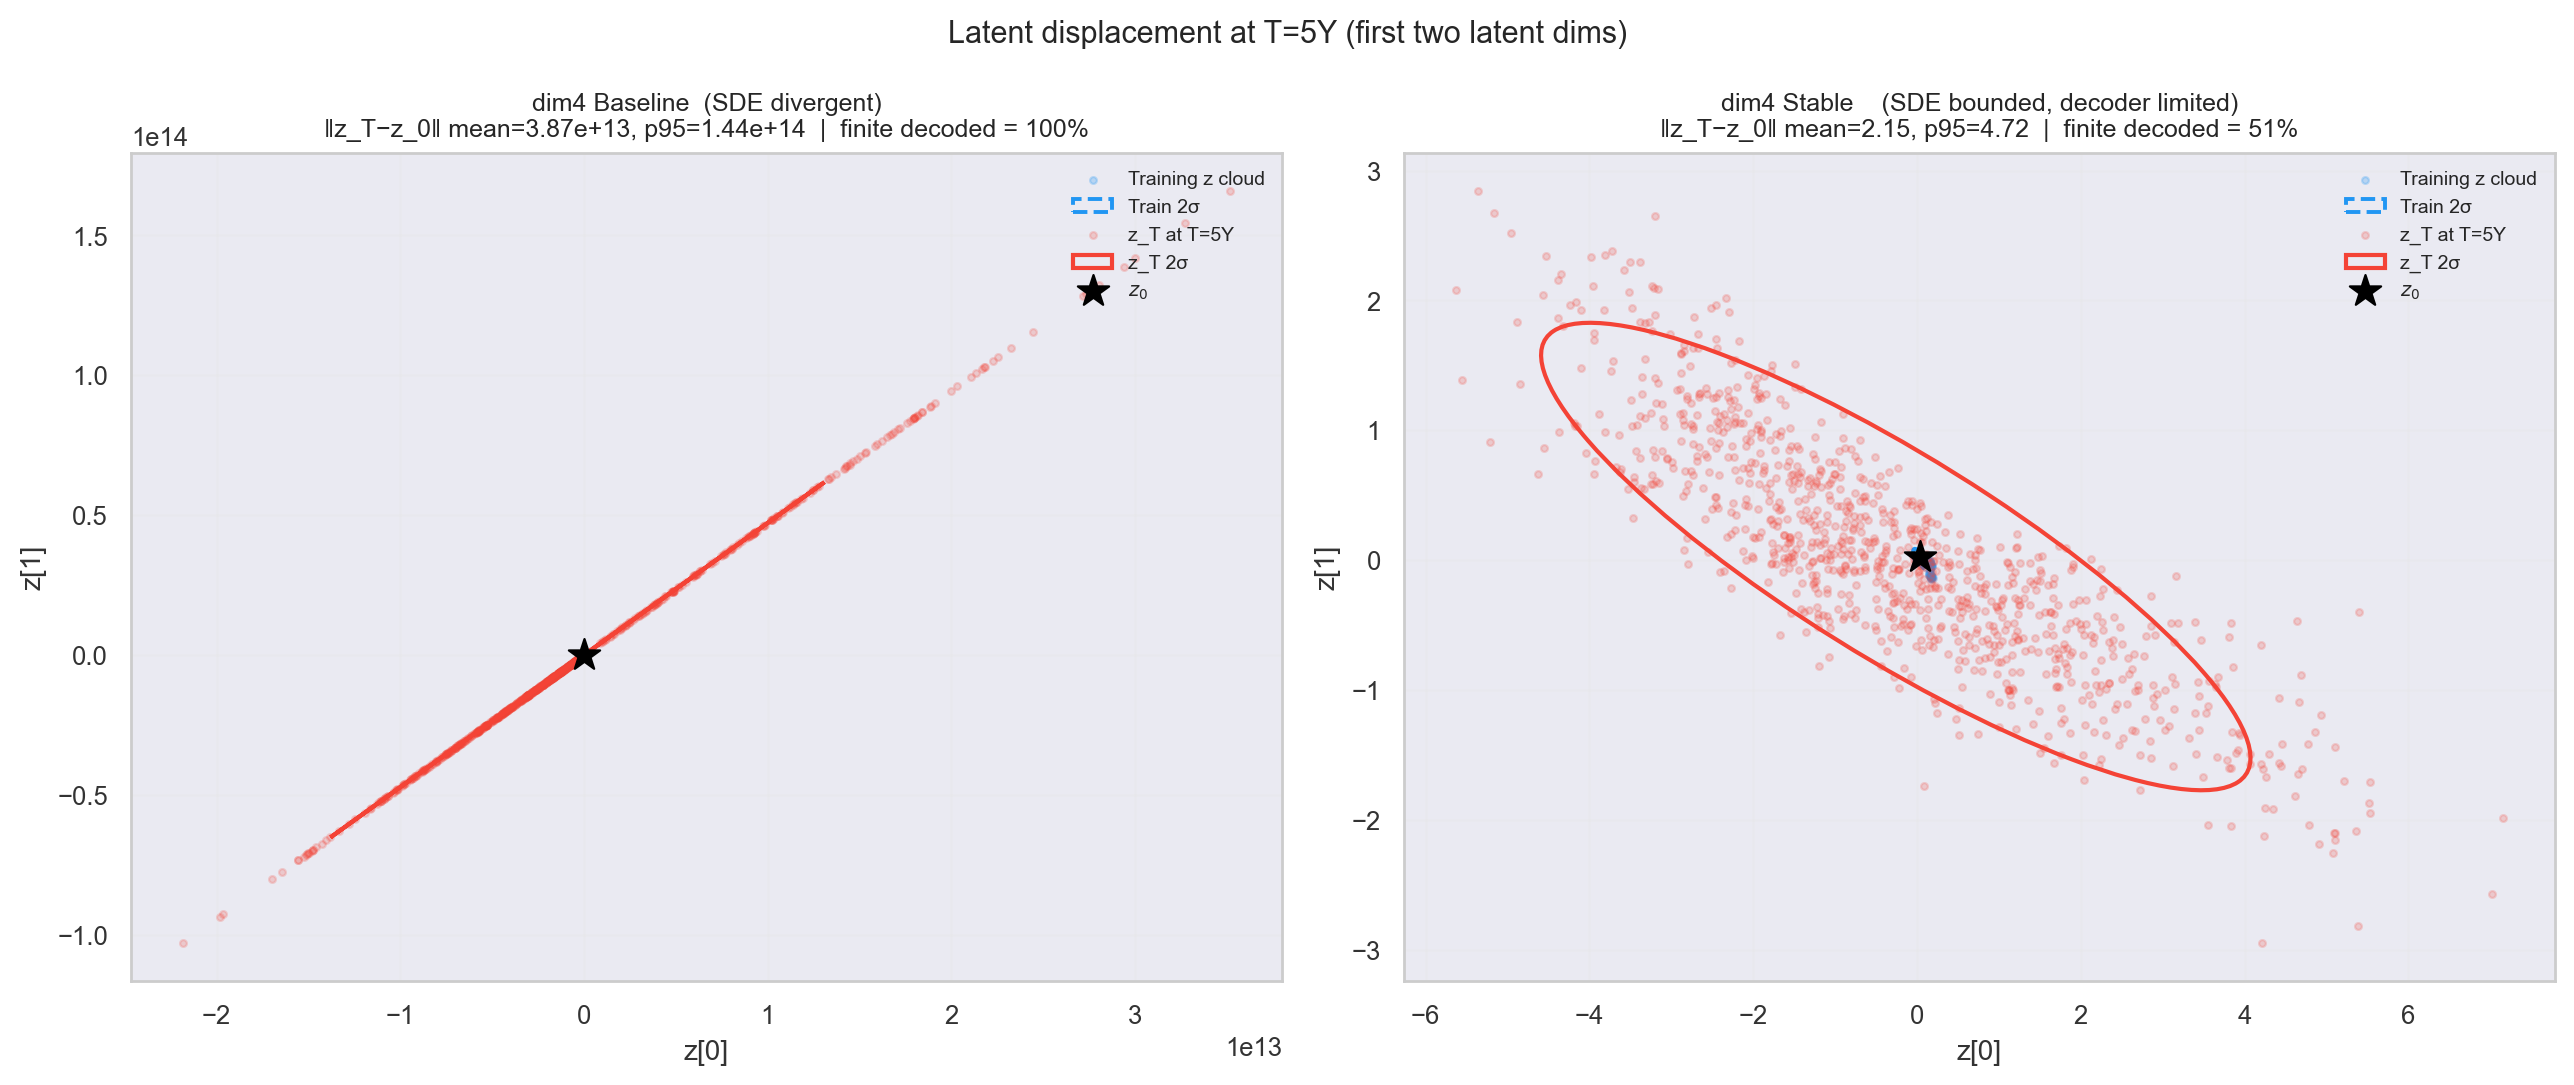
\includegraphics[width=\textwidth]{Figures/Pricing/fig_latent_displacement_scatter.png}
    \caption{Simulated $z_T$ at $T_e = 5$Y (red) overlaid on the encoded
    training cloud (blue), in the first two latent dimensions. Baseline's
    $z_T$ traces an unstable eigenvector at $\sim 10^{13}$; stable's $z_T$
    forms a well-behaved cloud of width $\sim 5$ around $z_0$, but already
    much larger than the encoded cloud's std of $\approx 0.05$.}
    \label{fig:latent_displacement_scatter}
\end{figure}

\begin{table}[H]
\centering
\caption{Statistics of $\|z_T - z_0\|$ at $T_e = 5$Y under Euler--Maruyama simulation ($N=1000$ paths, $\Delta t = 1/12$ y) and the corresponding fraction of paths that decode to finite discount curves. The baseline SDE diverges by thirteen orders of magnitude; the stable SDE produces well-behaved displacements but the recon-only decoder cannot handle them.}
\label{tab:displacement_summary}
\small
\begin{tabular}{lrrrrr}
\toprule
Model & Mean & Median & p95 & Max & Finite \% \\
\midrule
\texttt{dim4\_baseline} & 3.87e+13 & 1.88e+13 & 1.44e+14 & 3.3e+14 & 100.0\% \\
\texttt{dim4\_stable} & 2.15 & 1.9 & 4.72 & 7.59 & 51.2\% \\
\bottomrule
\end{tabular}
\end{table}

\paragraph{H versus K: where the displacement comes from.}
Decomposing the full displacement into diffusion-only and drift-only
contributions (Table~\ref{tab:hk_decomposition}, with the drift-only
trajectory plotted in Figure~\ref{fig:drift_only_displacement}) localises
the simulation pathology in the baseline. With $H = 0$, the baseline drift
alone produces $\|z_T - z_0\| \sim 8.4e+03$ over five years; the
linear part of $K$ has positive eigenvalues, and the unstable eigenvector
absorbs the entire trajectory. The stable variant has all-negative
eigenvalues by construction, and the drift-only displacement stays at
$\|z_T - z_0\| \approx 0.14$. For stable, the realised
displacement is therefore essentially the diffusion contribution
(annualised one-step diffusion $\approx$4.61),
moderated by the mean-reverting drift acting as a restoring force.

\begin{figure}[H]
    \centering
    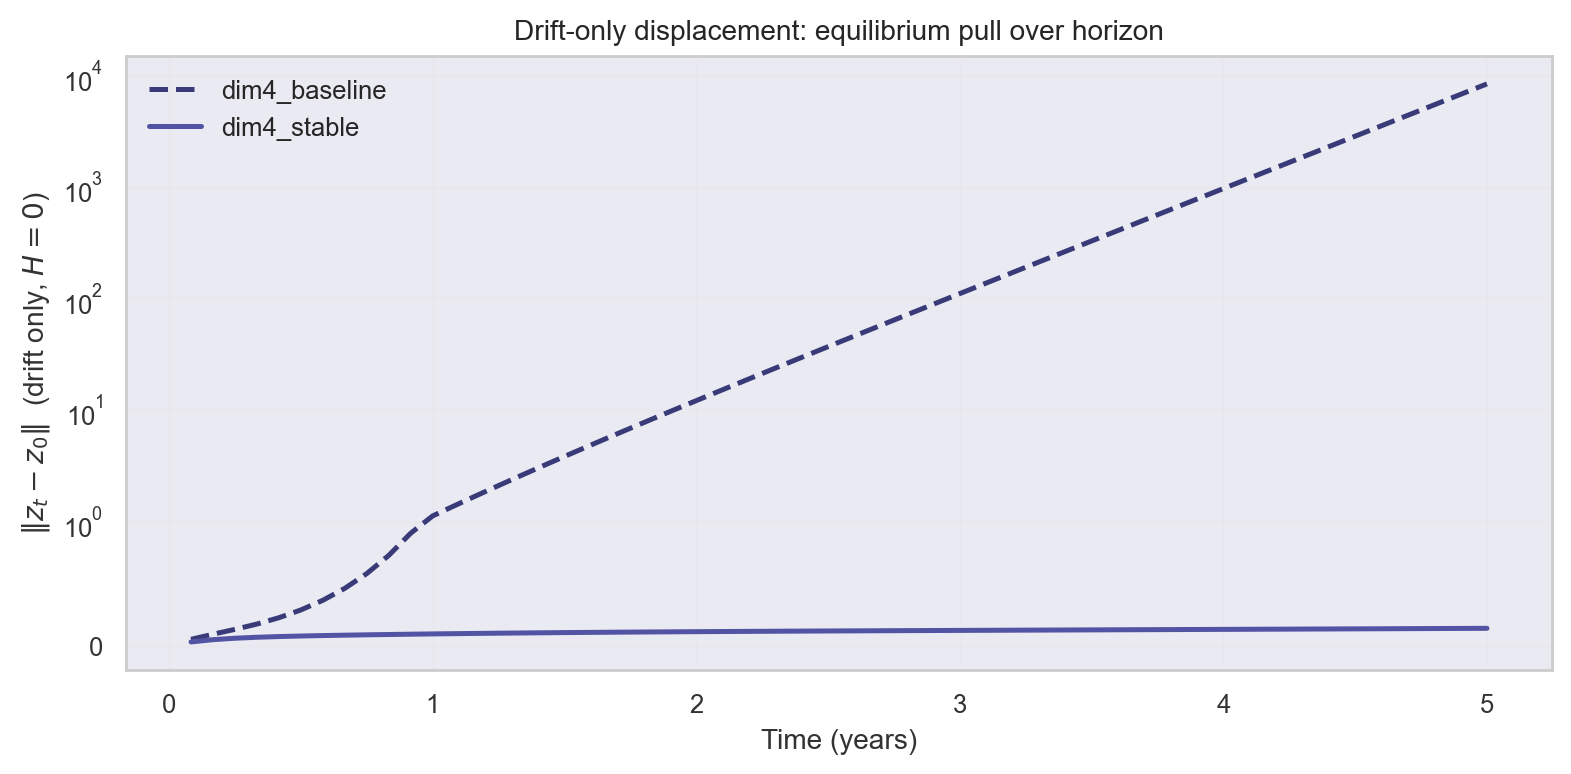
\includegraphics[width=0.75\textwidth]{Figures/Pricing/fig_drift_only_displacement.png}
    \caption{$\|z_t - z_0\|$ over time with $H = 0$ (drift only). Baseline grows
    exponentially along the unstable eigenvector; stable stays bounded.}
    \label{fig:drift_only_displacement}
\end{figure}

\begin{table}[H]
\centering
\caption{Decomposition of the 5-year displacement into diffusion and drift components for dim4 models. The \emph{Diff. annualised} column reports the one-step diffusion-only displacement scaled by $\sqrt{N_{\rm steps}}$ (approximate cumulative diffusion contribution). The \emph{Drift only} column reports $\|z_T - z_0\|$ with $H=0$ over $T = 5$Y. Stable's drift is bounded by mean reversion; baseline's drift alone explodes to $\sim 8\times 10^3$.}
\label{tab:hk_decomposition}
\small
\begin{tabular}{lrrrrr}
\toprule
Model & $\|z_0 - z^*\|$ & $\bar{\sigma}_H$ & Diff. annualised & Drift only ($T=5$Y) & Full ($T=5$Y) \\
\midrule
\texttt{dim4\_baseline} & 0.178 & 0.967 & 3.956 & 8.37e+03 & 3.87e+13 \\
\texttt{dim4\_stable} & 9.527 & 1.054 & 4.613 & 0.14 & 2.15 \\
\bottomrule
\end{tabular}
\end{table}

\paragraph{An apparent paradox in the stable variant.}
The stable equilibrium $z^* = -M^{-1} N_K$ for dim4 stable sits
$\|z^* - z_0\| \approx 9.5$ from a typical encoded EUR curve,
versus $\approx 0.18$ for baseline. One would expect a strong
mean-reverting drift with such a large equilibrium gap to dominate the
displacement, yet the drift-only contribution is only
$\approx 0.14$ over five years. The resolution is that
$(z^* - z_0)$ is almost entirely aligned with the slowest eigenvector of
$K$. Table~\ref{tab:eigenvector_alignment} shows the projection breakdown:
the slow eigenvector (timescale $\approx 1/|\lambda| \sim 600$ years)
absorbs essentially all of the misplacement, and over five years
$|1 - e^{\lambda T}|$ in that direction is below $0.01$. The misplacement
is structural — it sits in the direction the time-series fit cannot
constrain — but its dynamic effect at pricing-relevant horizons is small.

\begin{table}[H]
\centering
\caption{Eigenvector alignment of $(z^* - z_0)$ for dim4 stable. The slowest eigenvalue ($|\lambda| \approx 0.002$) absorbs essentially all of the misplacement. Over $T = 5$Y the slow direction barely activates ($1 - e^{\lambda T} \approx 0.008$), so the equilibrium misplacement contributes $\approx 0.14$ to the realised displacement, despite $\|z^* - z_0\| \approx 9.5$.}
\label{tab:eigenvector_alignment}
\small
\begin{tabular}{rrrrrr}
\toprule
Mode & $\lambda$ & timescale (y) & $|a_i|$ & $|1-e^{\lambda T}|$ & contribution \\
\midrule
0 & -5.0763 & 0.2 & 0.068 & 1.0000 & 0.0675 \\
1 & -2.3136 & 0.4 & 0.021 & 1.0000 & 0.0208 \\
2 & -1.0441 & 1.0 & 0.093 & 0.9946 & 0.0921 \\
3 & -0.0016 & 610.5 & 9.526 & 0.0082 & 0.0777 \\
\bottomrule
\end{tabular}
\end{table}

\paragraph{Implications for joint training.}
Three conclusions follow. First, both the recon-only stable model and
the recon-only baseline model fail at pricing, but for different reasons:
baseline fails by SDE divergence, stable fails by decoder rejection of
moderate displacements. Second, the stable architecture solves the SDE
problem identified in
Chapter~\ref{chap:encoderdecodermodel}\footnote{Or whichever chapter
houses the stability analysis — adjust the label.}; the decoder problem
is what remains. Third, joint training closes precisely the remaining
gap: the pricing loss $\mathcal{L}_{\mathrm{price}}$ in
\eqref{eq:pricing_loss} backpropagates through $\mathcal{G}(z_T)$,
forcing the decoder to extend its working domain to the displacement
range the SDE actually visits. The eigenvector-alignment result also
suggests that adding a regulariser pulling $|\lambda_K|$ away from zero
is conceptually clean (it eliminates the slow direction in which $z^*$
can drift unconstrained) without being strictly necessary at pricing
horizons of $5$ to $10$ years.
